\documentclass[a4paper,11pt]{article}

\pdfminorversion=4

\usepackage{cmap}
\usepackage[utf8]{inputenc}
\usepackage[T1]{fontenc}
\usepackage{lmodern}
\usepackage{geometry}
\usepackage{graphicx}
\usepackage{amsmath}
\usepackage{amssymb}
\usepackage{xcolor}
\usepackage{tikz}
\usepackage{hyperref}

\geometry{margin=2.4cm}
\setlength{\parindent}{0pt}
\setlength{\parskip}{0.65em}
\setlength{\emergencystretch}{2em}
\renewcommand{\abstractname}{Zusammenfassung}
\renewcommand{\figurename}{Abbildung}

\usetikzlibrary{arrows.meta,positioning,fit}

\title{S202: Ebenenlayout als Architekturhypothese\\
  \large Paketordnung, lokale Platzierung und explizite Schnittkanten}
\author{Johannes Weigend}
\date{Entwurf, 24.~Mai~2026}

\begin{document}

\maketitle

\begin{abstract}
S202 visualisiert Softwarearchitektur als geschichtetes Layout. Die
entscheidende Aussage der Darstellung ist einfach: Ein Element, das ein
anderes Element benutzt, steht oberhalb des benutzten Elements. In realen
Java-Systemen sind Paketabh\"angigkeiten nicht direkt beobachtbar --- sie
entstehen implizit und k\"onnen technisch nur aus den Klassenabh\"angigkeiten
ermittelt werden. Paketordnung, lokale Platzierung und Zyklusbehandlung
m\"ussen daher getrennt berechnet werden. Dieses Dokument beschreibt das
konzeptionelle Modell: Aus aggregierten Klassenabh\"angigkeiten entsteht
eine Architekturhypothese f\"ur Pakete; konkrete Kanten, die dieser Ordnung
widersprechen, werden als Backedges markiert; Kanten in SCCs werden f\"ur
die Ordnungsberechnung geschnitten, bleiben aber als explizites Feedback
sichtbar. Konsistenzregeln dienen anschliessend als implementierungsneutrale,
ausf\"uhrbare Spezifikation der erzeugten Grafik.
\end{abstract}

\section{Motivation}

Die geschichtete Darstellung von Abh\"angigkeiten ist ein etabliertes Mittel
der Softwarevisualisierung. Die Grundidee ist einfach: Wer abh\"angig ist,
steht oben; wer genutzt wird, steht unten.

S202 verfolgt dasselbe Ziel, aber mit einem anderen Anspruch. Die Darstellung
soll dem Nutzer eine Architekturabstraktion liefern, die \emph{ohne Pfeile
auskommt} und trotzdem Klarheit \"uber die Struktur gibt. Die vertikale
Position eines Elements tr\"agt die Information --- nicht die einzelne Kante.
Kanten sind in grossen Systemen nicht lesbar; eine stabile Schichtung ist es.

Das Ziel ist ausdr\"ucklich die Visualisierung \emph{grosser Anwendungen}.
In realen Java-Systemen mit Tausenden von Klassen und Hunderten von Paketen
ist eine manuelle Architekturzuweisung nicht praktikabel. S202 leitet die
Schichtung automatisch aus den beobachteten Abh\"angigkeiten ab und macht
dabei die zugrundeliegende Architekturhypothese explizit und nachvollziehbar.

\section{Geltungsbereich}

Dieses Dokument beschreibt das konzeptionelle Modell des geschichteten
S202-Layouts. Es ist keine zeilengetreue Beschreibung der aktuellen
Implementierung. Die Implementierung ist eine konkrete Auspr\"agung dieses
Modells und kann angepasst werden, wo sie die konzeptionelle Struktur noch
nicht pr\"azise genug abbildet.

Der Text vermeidet deshalb absichtlich Details wie konkrete Schwellenwerte,
historische Sonderf\"alle oder interne Namen einzelner Checks. Entscheidend
ist die fachliche Aussage der Darstellung: Die Grafik soll erkl\"aren k\"onnen,
warum jedes sichtbare Element an seiner Position steht und warum jede Kante,
die der Ordnung widerspricht, sichtbar bleibt.

\section{Grundbegriffe}

Eine Klassenabh\"angigkeit wird als

\[
  A \to B
\]

geschrieben und bedeutet: Klasse oder Element $A$ benutzt Klasse oder
Element $B$. S202 ordnet Elemente auf Ebenen an. Kleinere Level liegen in
der Grafik niedriger, gr\"ossere Level liegen h\"oher.

Eine Abh\"angigkeit ist \emph{ordnungskonform}, wenn der Nutzer oberhalb des
benutzten Elements liegt:

\[
  A \to B \quad\Longrightarrow\quad level(A) > level(B).
\]

Diese Konvention gilt f\"ur Klassenlevel, Paketlevel und lokale UI-Level,
aber die Berechnung erfolgt in zwei getrennten Schritten.

Zuerst entsteht die Paketordnung: Aus den aggregierten Klassenabh\"angigkeiten
werden Paketgewichte berechnet. Daraus folgt eine stabile Anordnung der
Pakete und ihrer Subpakete, die unabh\"angig von einzelnen Klassen ist.

Danach werden die Klassen eingeordnet: Innerhalb jedes Containers werden
Klassen und sichtbare Subpakete anhand ihrer lokalen Abh\"angigkeiten
untereinander sortiert. Die Paketordnung bleibt dabei erhalten --- eine
einzelne Klasse kann die Reihenfolge der Pakete nicht verschieben.

Eine Kante, die aus einem niedrigeren Element in ein h\"oheres Element zeigt,
widerspricht der berechneten Ordnung. Im Folgenden heisst eine solche Kante
\emph{gegenl\"aufige Kante} oder \emph{Backedge}. Sie ist kein Zeichenfehler:
Sie ist ein Befund der Architekturhypothese.

\section{Das Layoutversprechen}

Abbildung~\ref{fig:s202-deps-overview} zeigt das Grundprinzip der
S202-Darstellung. Links ist ein azyklisches Beispiel zu sehen. Die Kette
\texttt{E -> A -> B -> D} ist ordnungskonform:

\[
  L(E)=3,\quad L(A)=2,\quad L(B)=1,\quad L(D)=0.
\]

Der Nutzer steht jeweils \"uber dem benutzten Element. Die Abh\"angigkeit ist
damit unmittelbar aus der vertikalen Ordnung lesbar.

Rechts ist ein zyklisches Beispiel zu sehen. Die gestrichelten Kanten sind
keine zuf\"alligen Layoutfehler. Sie sind ausgew\"ahlte Teilkanten von SCCs,
die S202 f\"ur die Ebenenberechnung schneidet, um Zyklen aufzubrechen und
dabei die Architekturhypothese zu erhalten. Die Abh\"angigkeit wird dadurch
nicht gel\"oscht. Sie bleibt als explizite Schnittkante sichtbar.

\begin{figure}[htbp]
  \centering
  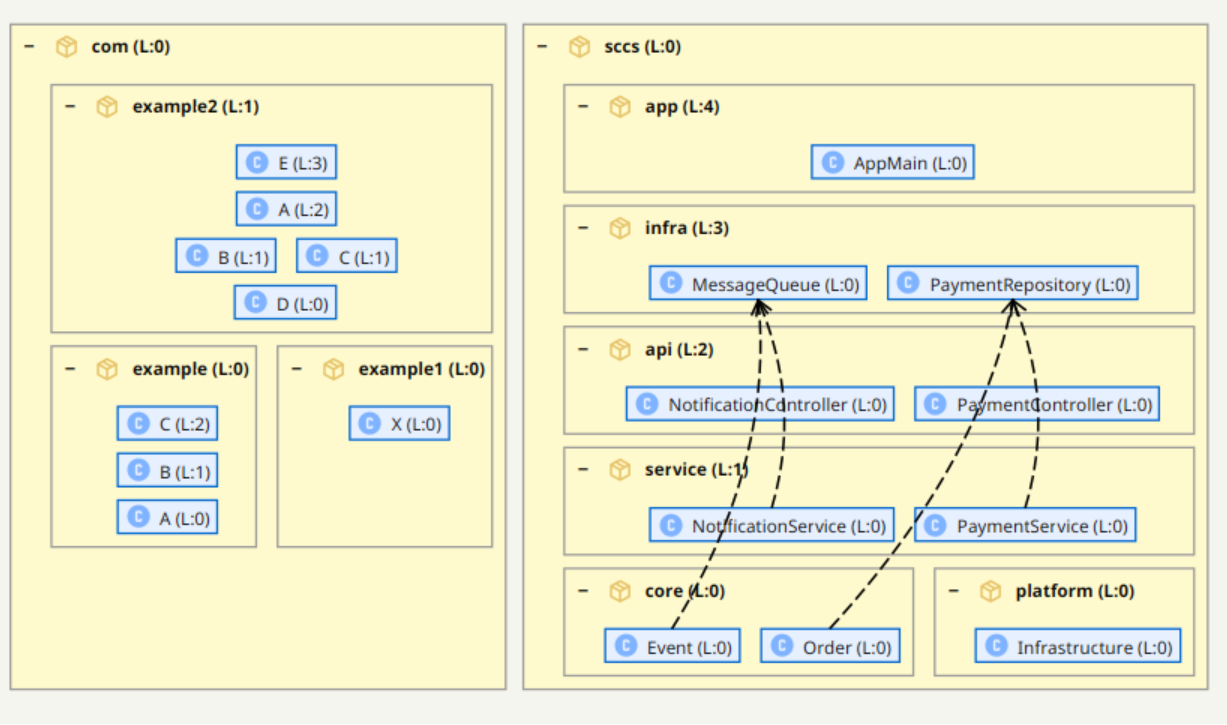
\includegraphics[width=\textwidth]{figures/S202-Dependencies.png}
  \caption{Das Layoutversprechen von S202.
  \textbf{Links:} ein azyklisches Beispiel. Levelwerte wachsen nach oben:
  \texttt{D} liegt auf Level~0, \texttt{B} und \texttt{C} auf Level~1,
  \texttt{A} auf Level~2 und \texttt{E} auf Level~3. Die Kette
  \texttt{E -> A -> B -> D} ist ordnungskonform.
  \textbf{Rechts:} ein zyklisches Beispiel. Die gestrichelten Kanten sind
  geschnittene Teilkanten von SCCs. Sie werden aus der Ordnungsberechnung
  entfernt, bleiben aber als explizite Feedback-Kanten sichtbar.}
  \label{fig:s202-deps-overview}
\end{figure}

Das Layoutversprechen lautet damit nicht: Die Grafik findet eine sch\"one
Anordnung. Es lautet: Die Grafik macht die Architekturhypothese nachvollziehbar.
Ordnungskonforme Abh\"angigkeiten passen zur Levelordnung. Kanten, die nicht
zur Levelordnung passen, verschwinden nicht stillschweigend, sondern werden
klassifiziert und sichtbar gemacht.

\section{Architekturhypothese aus Klassenabh\"angigkeiten}

S202 beobachtet keine direkten Paketabh\"angigkeiten als Prim\"ardaten. Das
Werkzeug kennt zun\"achst nur Klassen und Klassenabh\"angigkeiten. Eine
Paketbeziehung ist daher immer eine abgeleitete Aussage.

F\"ur zwei Pakete $P$ und $Q$ summiert S202 die Abh\"angigkeiten von Klassen in
$P$ zu Klassen in $Q$. Dasselbe geschieht in der Gegenrichtung. Dadurch
entstehen gewichtete Beziehungen:

\[
  w(P,Q)
  \qquad\text{und}\qquad
  w(Q,P).
\]

Dominieren die Abh\"angigkeiten von $P$ nach $Q$, dann interpretiert S202
$P$ als Nutzerpaket und $Q$ als tiefer liegendes, genutztes Paket:

\[
  w(P,Q) > w(Q,P)
  \quad\Longrightarrow\quad
  level(P) > level(Q).
\]

Diese Aussage ist eine Architekturhypothese, keine absolute Wahrheit. Sie
sagt: Nach den beobachteten Klassenabh\"angigkeiten ist es plausibel, $P$
oberhalb von $Q$ einzuordnen. Die sp\"atere lokale Platzierung darf diese
Hypothese nicht unbemerkt umdeuten.

Der entscheidende konzeptionelle Schritt ist, dass S202 die Paketbeziehungen
als \emph{eigenst\"andigen Graphen} behandelt --- einen Paketbaum, der
unabh\"angig von den einzelnen Klassen existiert. Dieser Baum entsteht aus
den aggregierten Gewichten und liefert eine stabile Ordnung. Erst diese
Stabilit\"at macht das Schneideproblem in zyklischen Klassengraphen l\"osbar:
Weil die Paketordnung feststeht, ist klar, welche Kanten gegen sie laufen
--- und genau diese werden als Kandidaten f\"ur den Schnitt betrachtet.

Sind die Gewichte in beiden Richtungen gleich gro\ss{},

\[
  w(P,Q) = w(Q,P),
\]

dann liefert die Hypothese keine Ordnung zwischen $P$ und $Q$. Beide
Pakete sind echte Peers: Sie nutzen einander gleich stark, und keine
Richtung dominiert. S202 l\"asst solche Paare auf demselben Level und
schneidet keine Kante zwischen ihnen. Das Ergebnis ist ein gemeinsames
SCC-Level, das die Symmetrie der Abh\"angigkeit ehrlich abbildet.

\section{Zyklen und Schnittkanten}

Zyklen sind der Grund, warum die Ebenenberechnung nicht als einfacher
Durchlauf \"uber alle Elemente funktioniert. In einem Zyklus k\"onnen nicht
alle Kanten gleichzeitig ordnungskonform sein. S202 muss daher entscheiden,
welche Kanten f\"ur die Ordnungsberechnung ignoriert werden, ohne sie aus dem
Modell oder aus der Grafik zu entfernen.

Ausgangspunkt ist die bereits berechnete Paketordnung. Eine konkrete
Klassenabh\"angigkeit wird als Backedge markiert, wenn sie aus einem Paket
kommt, das die Architekturhypothese niedriger eingeordnet hat, und in ein
h\"oher eingeordnetes Paket zeigt.

Ist eine solche Backedge Teil einer SCC, wird sie f\"ur die
Ordnungsberechnung geschnitten. Das Schneidekritierium ist dabei pr\"azise:
Geschnitten wird die Kante mit dem gr\"ossten Levelunterschied zwischen
Quell- und Zielpaket --- also die Kante, die am st\"arksten gegen die
Architekturhypothese l\"auft. Abbildung~\ref{fig:cut-rule} zeigt ein
Beispiel: Die Kante \texttt{core $\to$ api} \"uberspringt zwei Level
(von~0 nach~2) und ist damit die eindeutige Schnittkante. Eine Kante
\texttt{core $\to$ service} h\"atte nur einen Level \"ubersprungen und
w\"are nachrangig.

\begin{figure}[htbp]
  \centering
  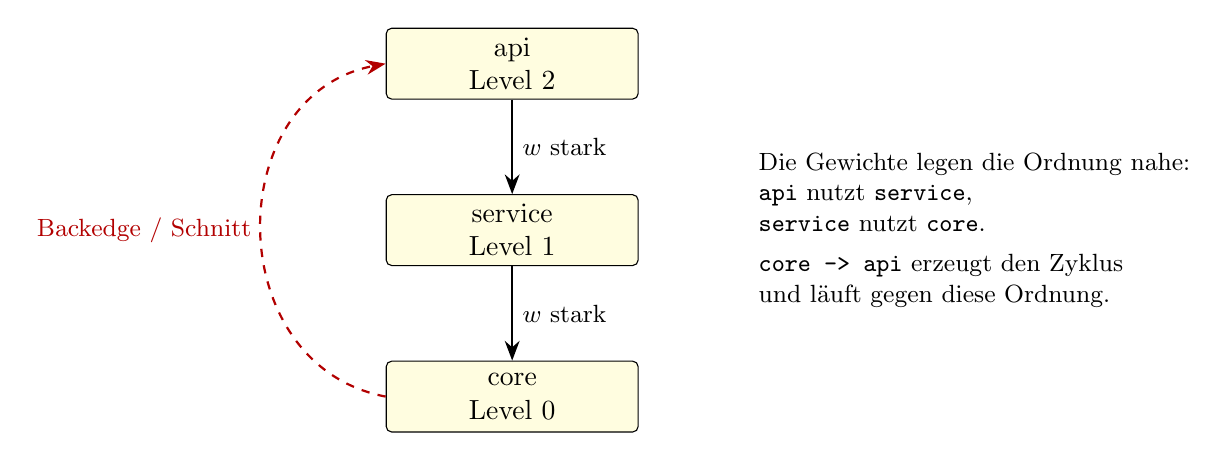
\begin{tikzpicture}[
      pkg/.style={
        draw,
        rounded corners=2pt,
        minimum width=3.2cm,
        minimum height=0.9cm,
        align=center,
        fill=yellow!12
      },
      dep/.style={-{Stealth[length=2.5mm]}, thick},
      cut/.style={-{Stealth[length=2.5mm]}, thick, dashed, red!70!black},
      note/.style={align=left, font=\small}
    ]
    \node[pkg] (api) {api\\Level 2};
    \node[pkg, below=1.2cm of api] (service) {service\\Level 1};
    \node[pkg, below=1.2cm of service] (core) {core\\Level 0};

    \draw[dep] (api) -- node[right, font=\small] {$w$ stark} (service);
    \draw[dep] (service) -- node[right, font=\small] {$w$ stark} (core);
    \draw[cut] (core.west) .. controls +(-2.1,0.4) and +(-2.1,-0.4) ..
      node[left, font=\small, text=red!70!black] {Backedge / Schnitt} (api.west);

    \node[note, right=1.4cm of service] (text) {
      Die Gewichte legen die Ordnung nahe:\\
      \texttt{api} nutzt \texttt{service},\\
      \texttt{service} nutzt \texttt{core}.\\[0.4em]
      \texttt{core -> api} erzeugt den Zyklus\\
      und l\"auft gegen diese Ordnung.
    };
  \end{tikzpicture}
  \caption{Schematische Schnittregel. Die Paketordnung entsteht aus
  aggregierten Klassenabh\"angigkeiten. Eine konkrete Abh\"angigkeit aus
  \texttt{core} nach \texttt{api} l\"auft von Level~0 nach Level~2 und damit
  gegen die Architekturhypothese. Ist diese Kante Teil einer SCC, wird sie
  f\"ur die Ordnungsberechnung geschnitten und bleibt als Schnittkante
  sichtbar.}
  \label{fig:cut-rule}
\end{figure}

Der Schnitt hat eine enge Bedeutung: Er entfernt die Kante nur aus dem Graphen,
auf dem die Level berechnet werden. Die reale Abh\"angigkeit bleibt erhalten.
Gerade dadurch wird die Darstellung ehrlich: Der Zyklus wird f\"ur die
Berechnung aufgebrochen, aber seine Ursache bleibt sichtbar.

\section{Lokale Platzierung}

Die Paketordnung beantwortet die Frage, welche Pakete nach der
Architekturhypothese oberhalb oder unterhalb anderer Pakete liegen. Sie
beantwortet aber nicht automatisch, wo eine Klasse innerhalb ihres sichtbaren
Elternpakets stehen soll.

Daf\"ur verwendet S202 eine lokale Platzierung. Innerhalb eines Containers
werden nur die direkten Geschwister betrachtet: Klassen und sichtbare
Subpakete, die um eine Position im selben Elternpaket konkurrieren. Aus den
Klassenabh\"angigkeiten zwischen diesen Geschwistern entsteht ein lokaler
Graph. Auf diesem Graphen werden lokale UI-Level berechnet.

Die lokale Platzierung darf die Paketarchitektur nicht neu definieren. Wenn
die Architekturhypothese ein Subpaket unterhalb eines anderen Containers sieht,
darf ein lokaler Sortierschritt diese Aussage nicht stillschweigend umkehren,
nur weil dadurch einige Linien k\"urzer oder weniger gegenl\"aufig aussehen.
Layout ist hier der Architekturhypothese untergeordnet.

Das ist der Grund f\"ur die Trennung der Begriffe:

\begin{itemize}
  \item Klassenlevel beschreiben die Ordnung im Klassenabh\"angigkeitsgraphen.
  \item Paketlevel beschreiben die aus Klassenabh\"angigkeiten aggregierte
        Architekturhypothese f\"ur Pakete.
  \item Lokale UI-Level beschreiben die sichtbare Position innerhalb eines
        konkreten Containers.
\end{itemize}

Alle drei verwenden dieselbe Grundidee: Nutzer stehen h\"oher als das
genutzte Element. Sie d\"urfen aber nicht zu einem einzigen globalen Level
vermischt werden.

\section{Konsistenzregeln als ausf\"uhrbare Spezifikation}

Konsistenzregeln waren in der Entwicklung von S202 nicht nur Testcode. Sie waren
die implementierungsneutrale Formulierung dessen, was eine konsistente Grafik
bedeuten muss.

Der Layoutalgorithmus erzeugt Modell, Level, Kantenklassifikationen und
sichtbare Reihenfolge. Die Konsistenzregeln werden danach gepr\"uft. Sie
schneiden keine Kanten, verschieben keine Elemente und optimieren kein Layout.
Sie pr\"ufen, ob die fertige Grafik ihre eigene Architekturhypothese einh\"alt.

Der Vorteil dieser Formulierung liegt in der Redundanz. Eine Konsistenzregel muss
nicht wissen, mit welchen internen Schritten der Layoutalgorithmus zu seinem
Ergebnis gekommen ist. Sie kann unabh\"angig implementiert werden und nur das
fertige Ergebnis lesen. Dadurch pr\"uft ein zweiter Codepfad dieselbe fachliche
Aussage.

Konzeptionell reichen drei Konsistenzregeln:

\begin{enumerate}
  \item Ordnungskonforme Abh\"angigkeiten erf\"ullen
        $level(A) > level(B)$.
  \item Eine nicht ordnungskonforme Kante verschwindet nicht. Sie ist als
        Backedge, SCC-Kante, Schnittkante oder Verletzung klassifiziert.
  \item Die sichtbare UI-Ordnung stimmt mit dem Modell \"uberein: Die
        Paketordnung aus der Architekturhypothese und die lokale Einordnung
        der Klassen innerhalb ihrer Container sind konsistent dargestellt.
\end{enumerate}

Die aktuelle Implementierung zerlegt diese Konsistenzregeln in vier konkrete
Checks:

\begin{description}
  \item[R1] Pr\"uft Konsistenzregel~1 f\"ur Klassenabh\"angigkeiten: Jede
        nicht als Backedge markierte Kante $A \to B$ muss
        $level(A) > level(B)$ erf\"ullen.
  \item[R2] Pr\"uft Konsistenzregel~1 f\"ur Pakete in derselben SCC: Peers
        ohne dominante Abh\"angigkeitsrichtung erhalten denselben Level.
  \item[R3] Pr\"uft Konsistenzregel~1 f\"ur Paketabh\"angigkeiten: F\"ur jede
        gewichtete Paketkante mit $w(P,Q) > w(Q,P)$ muss
        $level(P) > level(Q)$ gelten.
  \item[R4] Pr\"uft Konsistenzregel~2: Jede Abh\"angigkeit tr\"agt eine
        Klassifikation (NORMAL, VIOLATION, INTRA\_SCC). Kanten ohne
        Klassifikation sind ein Implementierungsfehler.
\end{description}

Konsistenzregel~3 (Level-Tupel-Vergleich bei verschachtelten UI-Elementen)
wird durch R1 und R3 in Teilen abgedeckt, ist aber noch kein vollst\"andiger
maschineller Check. Sie gilt konzeptionell als Ziel der Darstellung.

\section{Umsetzung in S202}

Aus dem konzeptionellen Modell ergibt sich eine klare Pipeline:

\begin{enumerate}
  \item Klassenabh\"angigkeiten aus dem analysierten Code lesen.
  \item Paketgewichte aus Klassenabh\"angigkeiten aggregieren.
  \item Aus den Paketgewichten eine Architekturhypothese berechnen
        (Paketordnung).
  \item Klassenlevel bestimmen: Zyklen im Klassengraphen werden entlang
        der Architekturhypothese geschnitten. Eine Kante $A \to B$ in einem
        Zyklus ist eine Schnittkante, wenn $pkgLevel(A) < pkgLevel(B)$.
        F\"ur Zyklen innerhalb gleich-levelliger Pakete greift die
        Grad-Heuristik als Fallback.
  \item Kanten, die nach Schritt~4 gegen die berechnete Ordnung laufen,
        als Backedges klassifizieren und sichtbar halten.
  \item Lokale UI-Level pro sichtbarem Container berechnen.
  \item Die fertige Grafik durch Konsistenzregeln pr\"ufen (R1--R4).
\end{enumerate}

\section{Zusammenfassung}

S202 macht die Architekturhypothese sichtbar: Wer wen benutzt, bestimmt
die vertikale Position --- nicht Kriterien wie kurze Kanten oder wenige
Kreuzungen. Diese Hypothese entsteht aus Klassenabh\"angigkeiten,
die zu Paketgewichten aggregiert werden. Daraus folgt eine Paketordnung.
Konkrete Kanten, die gegen diese Ordnung laufen, werden als Backedges
sichtbar. Sind sie Teil einer SCC, werden sie f\"ur die Ordnungsberechnung
geschnitten, aber nicht aus dem Modell entfernt.

Die zentrale Qualit\"at der Darstellung ist damit nicht, dass alle Linien
unauff\"allig aussehen. Die zentrale Qualit\"at ist Nachvollziehbarkeit: Jede
sichtbare Abweichung von der Ordnung muss erkl\"art werden k\"onnen.

\end{document}
